%!TEX root = ../thesis.tex
\section{組み立て}
組み立てたロボットアームの全体図を図\ref{fig:arm}に示す.また,寸法等の仕様を表\ref{tab:arm}に示す.組み立て時間は,約1時間である.
\begin{figure}[h]
  \centering
  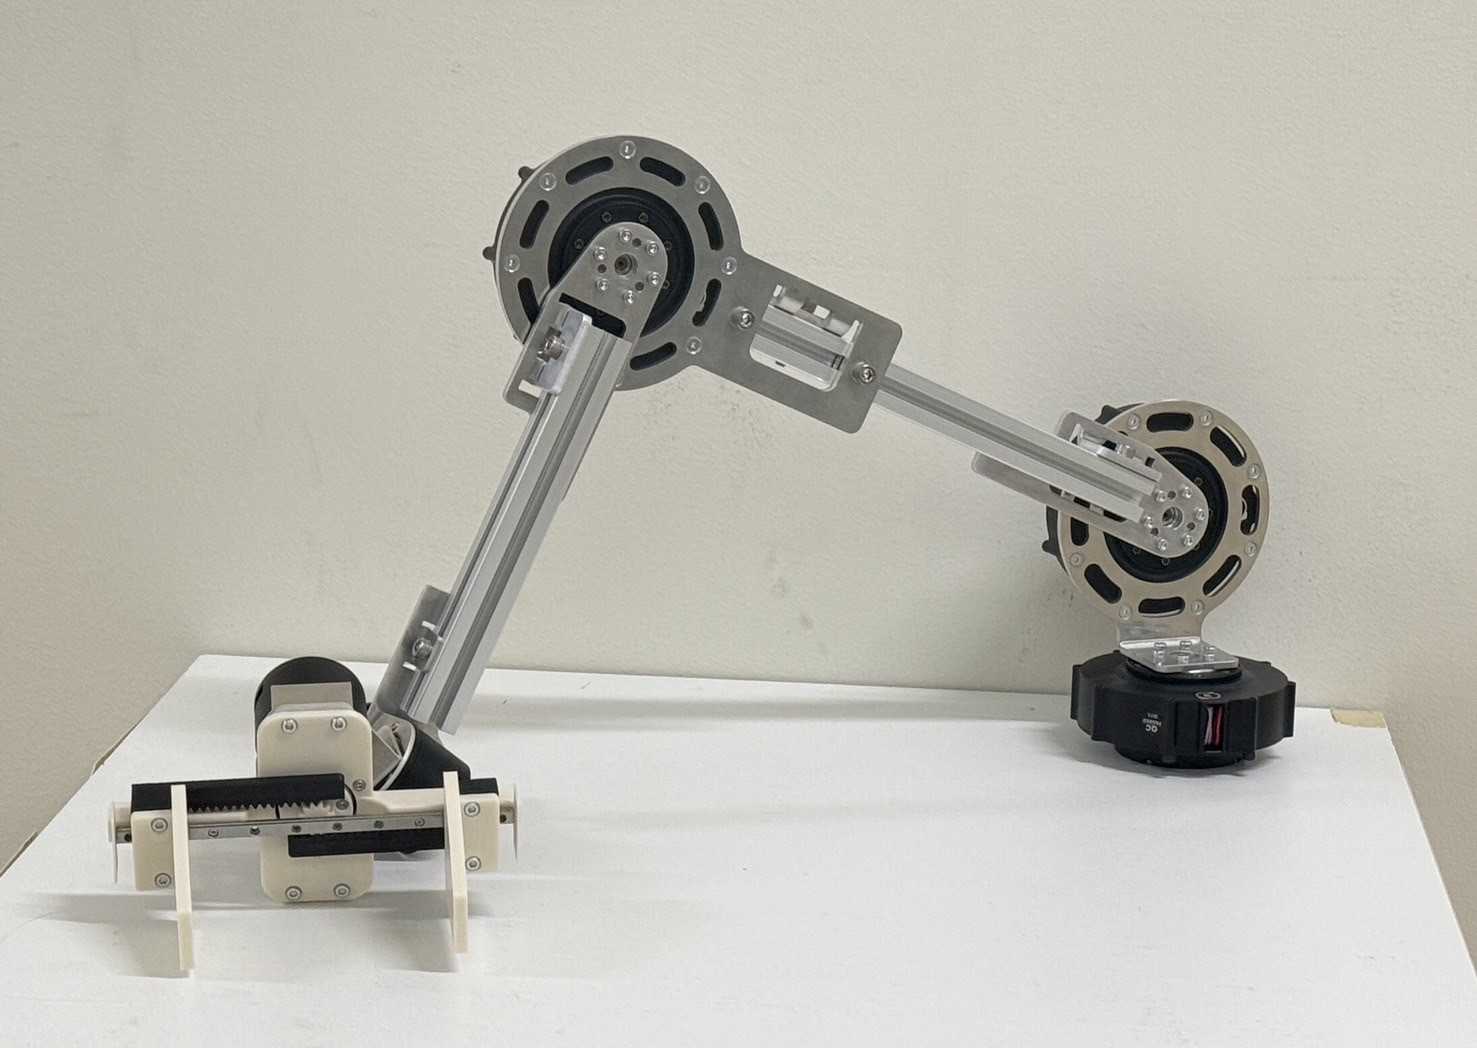
\includegraphics[width=10cm]{images/product/arm.jpg}
  \caption{Assembled robot arm}
  \label{fig:arm}
\end{figure}
\begin{table}[h]
  \centering
  \caption{Specifications of the robot arm}
  \begin{tabular}{ll}
  \hline
  Weight    & 2.2 kg                \\
  Length    & 760 mm                \\
  Materials & A5052, A6063S-T5, ASA \\ \hline
  \end{tabular}
  \label{tab:arm}
\end{table}

\newpage